\newcommand{\qcodeedit}{QCodeEdit}
\newcommand{\qtermwidget}{QTermWidget}
\newcommand{\stdout}{\texttt{stdout}}
\newcommand{\stderr}{\texttt{stderr}}

\section{Contexte initial}

    \subsection{État de l'art : \coqide{}}

        \subsubsection{Pas vraiment user-friendly}

        \coqide{} possède de nombreux défauts mineurs qui n'apparaissent pas au premier coup d'\oe{}il, mais après une utilisation fréquente de ce logiciel.
        On donne ici une liste de tels détails :
        \begin{itemize}
          \item L'impossibilité de fermer une fenêtre active : il faut sélectionner un autre onglet et effectuer une validation de code ;
          \item L'impossibilité d'ouvrir un fichier temporaire : il faut obligatoirement sauvegarder le nouveau fichier ;
          \item Une gestion calamiteuse de la coloration des fonctions de recherche et de remplacement : la coloration qui persiste ;
          \item L'impossibilité de copier-coller depuis un autre cadre que celui d'édition ;
          \item L'absence de coloration des délimiteurs ouvrants et fermants correspondants (parenthèses, etc.) ;
          \item Le cruel manque d'outils complémentaires que tout IDE devrait proposer : console, bibliothèque, etc. ;
          \item Divers bugs de l'éditeur (liés au copier-coller) ;
          \item Des bugs d'affichage incompréhensibles, sans doutes liés au \emph{binding} OCaml-GTK ;
          \item Le manque de personnalisation de l'interface\footnote{Ah, cette couleur, cette couleur !}.
        \end{itemize}

        On peut en outre constater d'autre défauts de conceptions plus importants, tels qu'une gestion des \emph{thread} catastrophique\footnote{\coqtop{} et \coqide{} sont si intimement liés que tout plantage de l'un induit un plantage de l'autre...}, et ce qui en découle, l'impossibilité de valider plusieurs documents à la fois.
			
        \subsubsection{Très opaque}

		En effet, le code de \coqide{} n'est pas très accessible, sa structure pas évidente, et il aurait probablement fallu plus de temps à le comprendre qu'à le développer. Plus exactement :
		\begin{itemize}
			\item Il n'y a aucune information sur le code, à part une maigre trame de structure dans la documentation du code source, mais cela reste très léger
			\item Peu modulaire : Il n'y a aucune séparation entre \coqide{} et le noyau de \coq{}, et \coqide{} n'a pas de structure propre indépendante de \coq{}. (cf. Les détails de la discussion avec Vincent Gross).	
		\end{itemize}
		
	\subsection{Les besoins du projet Coquille}

		Mise à part la nécessité d'un IDE pour \coq{}, qui reprenne donc les principales fonctionnalités de \coqide{} à savoir l'édition et coloration, l'envoi d'instructions à \coqtop{} étape par étape et la récupération des résultats ou messages d'erreurs, nous sommes restés à l'écoute des attentes des autres Groupes de Travail (Work Package en Anglais (WP)) :
        
        \subsubsection{WP Apprentissage}

        Les besoins principaux concernaient l'apprentissage :
		\begin{itemize}
			\item La possibilité pour l'utilisateur de donner une preuve `type' ou `classique' au programme d'apprentissage, qui se chargera de parser le code et d'apprendre la preuve. En somme, cela revient à un bouton "Apprendre cette preuve" qui pourrait s'appliquer à une sélection de code, ou à un théorème en particulier.
			\item Offrir à l'utilisateut une proposition de preuve ou de tactique, par un bouton "Propositions" par exemple, qui s'en suivrait par une liste de tactiques disponibles et adéquates.
			\item On pourrait envisager des retours à l'apprentissage pour dire que la proposition a été fructueuse ou que au contraire, elle est complètement absurde.
		\end{itemize}
			
		\subsubsection{WP Preuves / Tactiques}
			Ce groupe a fourni des librairies et des tactiques sous forme de fichiers en langage \coq{} directement utilisables par des commandes \coq{}, donc il n'y avait a priori aucune attente de la part de ce WP.

    \subsection{Que faire $\ldots$}

        \subsubsection{Tenter de modifier \coqide{} ?}

            Ce n'était clairement pas envisageable.
            En effet, non seulement le code de \coqide{} est complètement opaque (il aurait fallu en comprendre la structure, les subtilités, gérer le dialogue avec \coq{} sans modularité) mais en plus cela ne nous semblait pas très formateur de reprendre son code.
            On aurait pu certes reprendre \coqide{} et le structurer d'avantage, mais cela aurait été monstrueusement long.
			
        \subsubsection{Créer des plugins pour les éditeurs classiques ?}

			Mise à part \coqide{}, il n'y a pas d'éditeur dédié à \coq{}. En admettant que l'on eût fait un plugin pour un éditeur classique (netbeans, code::blocks), il aurait été dûr de dialoguer avec \coqtop{}, et un plugin ne permet pas de faire un interpréteur. Or, il nous semble vital d'avoir un interpréteur à disposition lorsqu'on code en \coq{}.
			
        \subsubsection{Coder un IDE \textit{from scratch} ?}
        
			C'est l'alternative que nous avons choisie. 
			Tout d'abord, il sera plus facile de bien structurer le code et de séparer le dialogue avec \coq{}.
			Cela permet également d'intégrer facilement la communication avec les fonctionnalités proposées par l'apprentissage.
			De même gérer des détails comme la mise en page, la coloration, le "folding" de preuves, nous paraît plus facile si on reprend l'IDE à zéro.
			
			Enfin, dans le cadre d'un tel projet, il est plus formateur de coder un éditeur à partir de rien et de se poser les questions de comment on le code ou on le structure dans un but précis plutôt que de perdre du temps à modifier un éditeur que nous ne comprenons pas.

\section{Quelques choix à faire}

    \subsection{Le Langage utilisé}
    
		Après réflexions, il a été décidé d'utiliser le C++.
		
		Durant la première semaine du Projet, deux parties du WP IDE se sont affrontées en proposant un mini-éditeur codé soit en Java avec Swing soit en C++ avec Qt. 
		Au cahier des charges, ils devaient proposer : 
		\begin{itemize}
			\item l'édition de texte avec les menus basiques (copier, coller, etc)
			\item la coloration syntaxique (désactivable) des parenthèses et de certains mots clés
			\item un bouton ``insertion" qui insère du texte après le curseur
			\item un bouton pour sortir l'intégralité du texte dans une nouvelle fenêtre
		\end{itemize}
		Après comparaison sur des critères prédéfinis, il en est ressorti que les deux langages sont très similaires tant en rapidité de codage (ils ont une API pour dessiner les fenêtres chacun par exemple), en structure, et sont assez abordables.
		Les deux mini-IDE étaient équivalents à la différence que celui en C++ était plus rapide et montrait plus de flexibilité dans la coloration syntaxique.
		Le mini-IDE en java utilisait des bibliothèques annexes (JLex) pour la coloration syntaxique.
		
		Nous avons donc choisi (à peu de différences) le C++. S'ajoutait le fait que parmi nous plus de personnes étaient compétents en C++ et novices en Java.
    
    \subsection{Les Bibliothèques utilisées}
    
        \subsubsection{Qt}
        
            Qt nous a séduit pour la gestion des fenêtres.
			En effet, QtCreator facilite amplement la création de fenêtres, le code Qt est très clair, propre et structuré; le slots sont gérés proprements en comparaison avec gtk par exemple.
			D'autre part, la documentation est vraiment très abordables de sorte que l'on a appris très rapidement sur le tas à se servir de Qt.
			
		\subsubsection{\qcodeedit}
			
			Nous avons passé beaucoup de temps à chercher une bibliothèque d'édition de texte fournissant un plugin de ``code folding".
			Il s'est avéré qu'il en existe peu, et \qcodeedit{} est l'une d'entre-elles.
			Nous nous sommes aperçu ensuite que cette bibliothèque, très puissante, permet de faire bien d'autres choses, ce qui nous a beaucoup aidé.
			
		\subsubsection{\qtermwidget}
			
			Pour intégrer un terminal à l'IDE, ce fût un peu le même combat que pour trouver \qcodeedit{}.
			Nous voulions un terminal qui puisse s'inclure dans un QWidget, et qui soit utilisable exactement comme un terminal UNIX.
		
    \subsection{Le dialogue avec \coq{}}
    
		Le choix s'est tout simplement restreint à \coqtop{}, car nous n'en avions pas trouvé d'autre.
        
\section{Les problèmes rencontrés}

    \subsection{Au niveau du langage}
    
		Qt et le C++ n'ont pas posé de problèmes majeurs. Nous étions déjà habitués à coder en C++, et les documentations de Qt et QtDesigner sont vraiment très abordables.
        
    \subsection{Au niveau des bibliothèques}
    
        Nous avons eu quelques petits problèmes de codage en utilisant la librairie \qcodeedit{}.

        Premièrement, c'est une bibliothèque plutôt destinée à être installée par l'utilisateur indépendamment de toute compilation.
        Nous voulions en inclure directement le code source dans notre programme, il nous a donc fallu batailler ferme.
        
        Ensuite, cette bibliothèque est un projet entier à elle seule, et apprendre à la maîtriser fût long car le code, quoique très bien documenté, reste du code écrit par quelqu'un d'autre, ce que tout le monde connaît comme très dur à relire.

        Au passage, un grand merci à Hugues Luc Bruant (ENSIMAG), responsable de cette bibliothèque, dont les réponses à nos mails étaient toujours rapides, claires et utiles, ce qui nous a sans nul doute sauvé de nombreuses mauvaises situations.
		
    \subsection{Au niveau du dialogue avec \coq{}}
    
        Ce furent les principaux problèmes, voici ceux qui nous ont pris le plus de temps.

        \subsubsection{La discrimination des erreurs}

        	Une réponse de \coqtop{}, qu'elle soit bonne ou mauvaise, est donnée sur \stdout{}. Seul le prompt passe par \stderr{}.
        	Et puisque \coqtop{} ne renvoie aucun autre signal, impossible \textit{a priori} de savoir si une réponse est une erreur ou pas.

        \subsubsection{Les réponses vides}

        	Certaines commandes de Galina ne renvoient absolument rien quand elles fonctionnent, et une erreur quand elles échouent.
        	\begin{itemize}
        		\item Si on attends une réponse pour pouvoir la discriminer en erreur ou non, on peut attendre très longtemps
        		\item Si on choisit un temps maximal d'attente, rien ne nous dit qu'une commande ne va pas prendre exactement 5 seconde de plus que ce laps de temps.
        	\end{itemize}

    	\subsubsection{L'annulation}

    	    Un véritable casse-tête $\ldots$
    	    
    	    Premièrement, la commande d'annulation d'une commande de base n'est pas la même selon que l'on est au sein d'une preuve ou non.
    	    
    	    Ensuite, certaines commandes sont purement inutiles et sont ignorées par \coqtop{}.
    	    C'est le cas de la commande \coqcode{Proof.}, qu'il ne faut surtout pas tenter d'annuler sous peine d'annuler la commande précédente.
    	    
    	    Enfin, dans certains cas, il est tout simplement impossible actuellement d'annuler une seule opération.
    	    D'après ces messieurs de l'INRIA eux-même, le seul moyen d'annuler la commande \coqcode{Qed.} validant un théorème nommé \coqcode{truc}, par exemple, est de faire \coqcode{Reset truc.}, puis de renvoyer une-à-une les commandes situées entre la définition de \coqcode{truc} et le fameux \coqcode{Qed}.
    	    Si jamais la preuve est longue, ou comporte des calculs longs pour l'ordinateur, c'est complètement insensé.
    	    
    	    Pire encore, dans le cas de preuves imbriquées, \coqcode{Reset truc} annule toutes les preuves jusqu'à revenir en mode Galina.
    	    
            Une solution envisagée était d'utiliser les commandes \coqcode{Write State} et \coqcode{Restore State} à chaque étape pour pouvoir revenir en arrière plus facilement.
            Seulement \coqtop{} est tellement surprenant que :
            \begin{itemize}
             	\item \coqcode{Write State} ne fait pas que sauvegarder l'état, il réinitialise \coqtop{}
             	\item \coqcode{Restore State} ne fonctionne pas du tout !
             \end{itemize}
		
		Nous avons donc contacté Vincent Gross (INRIA), et de cette discussion il ressort qu' « il n'y a à l'heure actuelle aucune séparation entre \coq{} et ses interfaces de communication (\coqtop{}, \coqide{}) », et que si on a du mal à travailler de cette manière, « c'est tout simplement parce qu'il n'existe aucune API ».
		Aucun moyen, donc, de faire notre propre interface sans faire des choses (très) sales.
				
\section{Le résultat actuel}

    \subsection{Ce que Coquille fait et que \coqide{} ne fait pas !}
    
        \subsubsection{Au niveau du code}
        
            \begin{itemize}
                \item Marquer les numéros de ligne (cf. Fig \ref{fig:lines})
                \item Le ``code folding" : replier des lignes de code en une seule pour améliorer la lisibilité (cf. Fig \ref{fig:folding})
                \item Des raccourcis clavier plus ``classiques", et personnalisables
                \item La possibilité de faire des ``Redo" après des ``Undo" (cf. Fig \ref{fig:redo})
            \end{itemize}
            \begin{figure}[ht]
                \begin{minipage}[b]{0.3\linewidth}
                    \centering
                    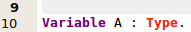
\includegraphics[scale=0.5]{../images/ide/lines.png}
                    \caption{La numérotation des lignes}
                    \label{fig:lines}
                \end{minipage}
                \hfill
                \begin{minipage}[b]{0.3\linewidth}   
	                \centering
	                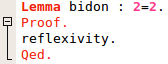
\includegraphics[scale=0.5]{../images/ide/folding.png}
	                \caption{Le ``code folding"}
	                \label{fig:folding}
                \end{minipage}
                \hfill
                \begin{minipage}[b]{0.3\linewidth}   
	                \centering
	                
\includegraphics[scale=0.5]{../images/ide/redo.png}
	                \caption{Le ``Redo"}
	                \label{fig:redo}
	            \end{minipage}
            \end{figure}
            
        \subsubsection{Au niveau du langage}

            \begin{itemize}
                \item La gestion de \coqcode{Ltac Debug} (cf. Fig \ref{fig:ltacdebug})
                C'est une interface que nous avons mis au point et qui permet de voir en détail l'exécution d'une tactique en \coq{}, avec une interface de parcours des résultats
                \item Gérer plusieurs instances de \coqtop{}, une par onglet ouvert, sans annuler tout à chaque changement d'onglet
                \item Un affichage des résultats en version classique ou $\LaTeX$-like (cf. Fig \ref{fig:unicode})
                \item L'action « Send / Unsend » d'envoi d'une commande est considérée comme une action comme les autres, donc « Undo / Redo » peut agir dessus
            \end{itemize}
            \begin{figure}[ht]
	            \centering
	            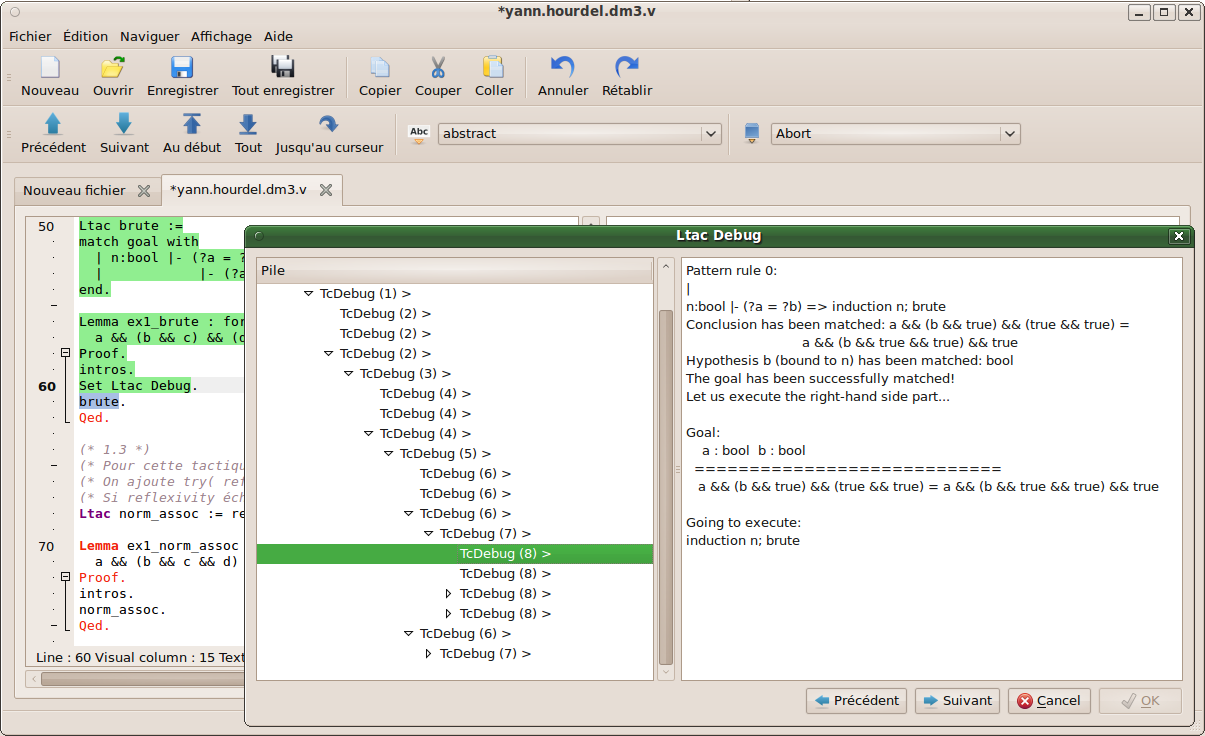
\includegraphics[scale=0.35]{../images/ide/ltacdebug.png}
	            \caption{Le mode Ltac Debug}
	            \label{fig:ltacdebug}
            \end{figure}
            \begin{figure}[ht]
	            \centering
	            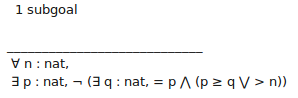
\includegraphics[scale=0.5]{../images/ide/unicode.png}
	            \caption{L'affichage $\LaTeX$-like}
	            \label{fig:unicode}
            \end{figure}
            
    \subsection{Ce que \coqide{} fait et que Coquille ne fait pas (encore)}
    
        \subsubsection{Au niveau du code}

            \begin{itemize}
                \item Lister les actions disponibles par click droit sur une hypothèse ou un but.
            \end{itemize}

        \subsubsection{Au niveau du langage}
        
            \begin{itemize}
                \item Le Proof Wizard.
                \item La gestions de la compilation et des exportations : \coqide{} permet de compiler / exporte un fichier sans passer par ligne de commande
            \end{itemize}

    \subsection{Ce que ni l'un ni l'autre ne font bien}

        \subsubsection{Au niveau du code}

            \begin{itemize}
                \item L'auto-complétion
            \end{itemize}

        \subsubsection{Au niveau du langage}
        
            \begin{itemize}
                \item La gestion de l'aide
                \item La gestion des « \coqcode{Write State} / \coqcode{Restore State} ».
                En théorie, la commande \coqcode{Write State} est censée sauvegarder l'état de l'interpréteur (variables, commandes envoyées, etc), tandis que \coqcode{Restore State} est censé restaurer cet état.
			    En pratique, \coqcode{Restore State} ne marche pas dans \coqtop{}, ce qui nous empêche de l'utiliser.
            \end{itemize}

\section{Les objectifs}

La majorité des objectifs que le WP IDE s'étaient fixés à l'origine ont été largement atteints puisqu'on dispose d'un IDE fonctionnel si on s'interdit la gestion de l'environnement (\coqcode{Write State} \& cie),  qui reprend \coqide{} avec plus de fonctionnalités et qui est plus pratique à utiliser dans l'optique du projet.

Il serait envisageable de continuer le projet si l'INRIA finit de développer une interface de dialogue avec \coq{} utilisable.
En attendant, on ne peut que corriger les bugs.

Au niveau de la distribution, nous avons déjà mis Coquille sous forme de paquets (\code{.deb} \& cie). Il nous reste donc principalement à distribuer et diffuser Coquille dans la communauté \coq{} et à y inclure un petit manuel d'utilisation. Un manuel programmeur basique est déjà mis à disposition.

